

%% AAPT Physics Olympiad F=ma Questions
%%----------------------------------------


%% PhysicsOlympiad 2015
%%----------------------------------------


%% PhysicsOlympiad 1999
%%----------------------------------------
\element{aapt}{ %% Olympiad-D1
\begin{question}{olympiad-1999-q28}
    Which of the following graphs would best represent the electric field of a hollow Van de Graff sphere as a function of distance from its center when it is charged to a potential of \SI{400 000}{\volt}?
    \begin{multicols}{2}
    \begin{choices}
        \AMCboxDimensions{down=-2.5em}
        \wrongchoice{
            \begin{tikzpicture}
                \begin{axis}[
                    axis y line=left,
                    axis x line=bottom,
                    axis line style={->},
                    xlabel={radius},
                    xtick=\empty,
                    ylabel={electric field},
                    ytick=\empty,
                    xmin=0,xmax=11,
                    ymin=0,ymax=11,
                    width=0.95\columnwidth,
                    very thin,
                ]
                \addplot[line width=1pt,domain=0:10]{ 10/x };
                \end{axis}
            \end{tikzpicture}
        }
        \wrongchoice{
            \begin{tikzpicture}
                \begin{axis}[
                    clip=false,
                    axis y line=left,
                    axis x line=bottom,
                    axis line style={->},
                    xlabel={radius},
                    xtick=\empty,
                    ylabel={electric field},
                    ytick=\empty,
                    xmin=0,xmax=11,
                    ymin=0,ymax=11,
                    width=0.95\columnwidth,
                    very thin,
                ]
                \addplot[line width=1pt,domain=0:1]{ 10 };
                \addplot[line width=1pt,domain=1:10]{ 10/x };
                \end{axis}
            \end{tikzpicture}
        }
        %% ANS is C
        \correctchoice{
            \begin{tikzpicture}
                \begin{axis}[
                    axis y line=left,
                    axis x line=bottom,
                    axis line style={->},
                    xlabel={radius},
                    xtick=\empty,
                    ylabel={electric field},
                    ytick=\empty,
                    xmin=0,xmax=11,
                    ymin=0,ymax=11,
                    width=0.95\columnwidth,
                    very thin,
                ]
                \addplot[line width=1pt,mark=\empty] plot coordinates { (0,0) (1,0) (1,10) };
                \addplot[line width=1pt,domain=1:10]{ 10/x };
                \end{axis}
            \end{tikzpicture}
        }
        \wrongchoice{
            \begin{tikzpicture}
                \begin{axis}[
                    axis y line=left,
                    axis x line=bottom,
                    axis line style={->},
                    xlabel={radius},
                    xtick=\empty,
                    ylabel={electric field},
                    ytick=\empty,
                    xmin=0,xmax=11,
                    ymin=0,ymax=11,
                    width=0.95\columnwidth,
                    very thin,
                ]
                \addplot[line width=1pt,mark=\empty] plot coordinates { (0,0) (1,10) };
                \addplot[line width=1pt,domain=1:10]{ 10/x };
                \end{axis}
            \end{tikzpicture}
        }
        \wrongchoice{
            \begin{tikzpicture}
                \begin{axis}[
                    axis y line=left,
                    axis x line=bottom,
                    axis line style={->},
                    xlabel={radius},
                    xtick=\empty,
                    ylabel={electric field},
                    ytick=\empty,
                    xmin=0,xmax=11,
                    ymin=0,ymax=11,
                    width=0.95\columnwidth,
                    very thin,
                ]
                \addplot[line width=1pt,mark=\empty] plot coordinates { (0,0) (1,10) (10,4) };
                \end{axis}
            \end{tikzpicture}
        }
    \end{choices}
    \end{multicols}
\end{question}
}

\newcommand{\aaptOlympiadZeroZeroQTwentyNine}{
\begin{tikzpicture}
    \node[draw,dashed,minimum width=4cm,minimum height=3cm] (A) at (0,0) {};
    %% lengths
    \node[rotate=90,anchor=south] at (A.west) {\SI{60}{\centi\meter}};
    \node[anchor=north] at (A.south) {\SI{80}{\centi\meter}};
    %% center, point X
    \draw[fill] (A.center) circle (1.5pt) node[anchor=west] {$X$};
    %% charges
    \draw[fill] (A.north west) circle (1.5pt) node[anchor=south east] {$Q_1$};
    \draw[fill] (A.south west) circle (1.5pt) node[anchor=north east] {$Q_2$};
    \draw[fill] (A.south east) circle (1.5pt) node[anchor=north west] {$Q_3$};
\end{tikzpicture}
}

\element{aapt}{ %% Olympiad-D1
\begin{question}{olympiad-2000-q29}
    %% Questions 29 and 30 refer to the following situation.
    Three electric charges ($Q_1$, $Q_2$ and $Q_3$) are arranged at three corners of a rectangle as shown in the diagram and each has a charge of \SI{-40}{\nano\coulomb}.
    \begin{center}
        \aaptOlympiadZeroZeroQTwentyNine
    \end{center}
    What is the magnitude of the net force on $Q_2$?
    \begin{multicols}{2}
    \begin{choices}
        \wrongchoice{\SI{1.4e-5}{\newton}}
        \wrongchoice{\SI{1.7e-5}{\newton}}
        \wrongchoice{\SI{4.2e-5}{\newton}}
      \correctchoice{\SI{4.6e-5}{\newton}}
        \wrongchoice{\SI{14.7e-5}{\newton}}
    \end{choices}
    \end{multicols}
\end{question}
}

\element{aapt}{ %% Olympiad-D1
\begin{question}{olympiad-2000-q30}
    %% Questions 29 and 30 refer to the following situation.
    Three electric charges ($Q_1$, $Q_2$ and $Q_3$) are arranged at three corners of a rectangle as shown in the diagram and each has a charge of \SI{-40}{\nano\coulomb}.
    \begin{center}
        \aaptOlympiadZeroZeroQTwentyNine
    \end{center}
    What would be the magnitude of the total electric field at center point $X$?
    \begin{multicols}{2}
    \begin{choices}
      \correctchoice{\SI{1440}{\newton\per\coulomb}}
        \wrongchoice{\SI{720}{\newton\per\coulomb}}
        \wrongchoice{\SI{360}{\newton\per\coulomb}}
        \wrongchoice{\SI{180}{\newton\per\coulomb}}
        \wrongchoice{\SI{90}{\newton\per\coulomb}}
    \end{choices}
    \end{multicols}
\end{question}
}


%% PhysicsOlympiad 1998
%%----------------------------------------
\element{aapt}{ %% Olympiad-D1
\begin{question}{olympiad-1998-q25}
    A charge is uniformly distributed through a volume of radius $a$.
    Which of the graphs below best represents the magnitude of the electric field as a function of distance from the center of the sphere?
    \begin{multicols}{2}
    \begin{choices}
        \AMCboxDimensions{down=-2.5em}
        \wrongchoice{
            \begin{tikzpicture}
                \begin{axis}[
                    axis y line=left,
                    axis x line=bottom,
                    axis line style={->},
                    xlabel={radius},
                    xtick={3},
                    xticklabels={$a$},
                    x label style={
                        at={(current axis.right of origin)},
                        anchor=north east,
                    },
                    ylabel={$E$ field},
                    ytick=\empty,
                    xmin=0,xmax=11,
                    ymin=0,ymax=11,
                    width=0.95\columnwidth,
                    very thin,
                ]
                \addplot[line width=1pt,domain=0:3]{5};
                \addplot[line width=1pt,domain=3:10]{45/x/x};
                \end{axis}
            \end{tikzpicture}
        }
        \wrongchoice{
            \begin{tikzpicture}
                \begin{axis}[
                    axis y line=left,
                    axis x line=bottom,
                    axis line style={->},
                    xlabel={radius},
                    xtick={3},
                    xticklabels={$a$},
                    x label style={
                        at={(current axis.right of origin)},
                        anchor=north east,
                    },
                    ylabel={$E$ field},
                    ytick=\empty,
                    xmin=0,xmax=11,
                    ymin=0,ymax=11,
                    width=0.95\columnwidth,
                    very thin,
                ]
                \addplot[line width=1pt,no marks] plot coordinates { (0,5) (3,5) (10,1) };
                \end{axis}
            \end{tikzpicture}
        }
        \wrongchoice{
            \begin{tikzpicture}
                \begin{axis}[
                    axis y line=left,
                    axis x line=bottom,
                    axis line style={->},
                    xlabel={radius},
                    xtick={3},
                    xticklabels={$a$},
                    x label style={
                        at={(current axis.right of origin)},
                        anchor=north east,
                    },
                    ylabel={$E$ field},
                    ytick=\empty,
                    xmin=0,xmax=11,
                    ymin=0,ymax=11,
                    width=0.95\columnwidth,
                    very thin,
                ]
                \addplot[line width=1pt,no marks] plot coordinates { (0,0) (3,0) (3,5) };
                \addplot[line width=1pt,domain=3:10]{45/x/x};
                \end{axis}
            \end{tikzpicture}
        }
        %% ANS is D
        \correctchoice{
            \begin{tikzpicture}
                \begin{axis}[
                    axis y line=left,
                    axis x line=bottom,
                    axis line style={->},
                    xlabel={radius},
                    xtick={3},
                    xticklabels={$a$},
                    x label style={
                        at={(current axis.right of origin)},
                        anchor=north east,
                    },
                    ylabel={$E$ field},
                    ytick=\empty,
                    xmin=0,xmax=11,
                    ymin=0,ymax=11,
                    width=0.95\columnwidth,
                    very thin,
                ]
                \addplot[line width=1pt,no marks] plot coordinates { (0,0) (3,5) };
                \addplot[line width=1pt,domain=3:10]{45/x/x};
                \end{axis}
            \end{tikzpicture}
        }
        \wrongchoice{
            \begin{tikzpicture}
                \begin{axis}[
                    axis y line=left,
                    axis x line=bottom,
                    axis line style={->},
                    xlabel={radius},
                    xtick={3},
                    xticklabels={$a$},
                    x label style={
                        at={(current axis.right of origin)},
                        anchor=north east,
                    },
                    ylabel={$E$ field},
                    ytick=\empty,
                    xmin=0,xmax=11,
                    ymin=0,ymax=11,
                    width=0.95\columnwidth,
                    very thin,
                ]
                \addplot[line width=1pt,no marks] plot coordinates { (0,0) (3,5) (10,1) };
                \end{axis}
            \end{tikzpicture}
        }
    \end{choices}
    \end{multicols}
\end{question}
}

\element{aapt}{ %% Olympiad-D1
\begin{questionmult}{olympiad-1998-q26}
    A free electron and a free proton are placed between two oppositely charged parallel plates.
    Both are closer to the positive plate than the negative plate.
    %% See diagram to the right.
    \begin{center}
    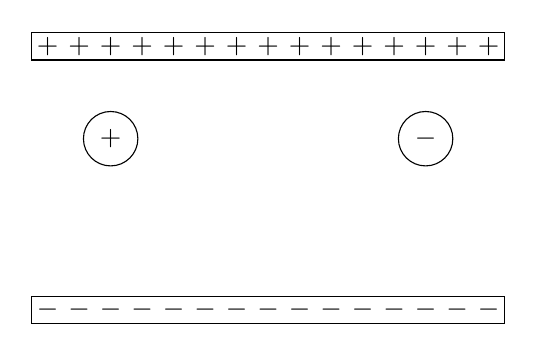
\begin{tikzpicture}
        %% Charges
        \node[draw,circle,anchor=center] at (+1,2) {$+$};
        \node[draw,circle,anchor=center] at (+5,2) {$-$};
        %% Top
        \draw (0,0) rectangle (6,-1em);
        \foreach \x in {2,6,...,58}
            \node[anchor=center] at (\x mm,3cm+0.5em) {$+$};
        %% Bottom
        \draw (0,3) rectangle (6,3cm+1em);
        \foreach \x in {2,6,...,58}
            \node[anchor=center] at (\x mm,-0.5em) {$-$};
    \end{tikzpicture}
    \end{center}
    Which of the following statements is true?
    \begin{choices}
        \wrongchoice{The force on the proton is greater than the force on the electron.}
      \correctchoice{The potential energy of the proton is greater than that of the electron.}
        \wrongchoice{The potential energy of the proton and the electron is the same.}
        %% A. I only B. II only C. III only D. I & II only E. I & III only
    \end{choices}
\end{questionmult}
}


%% PhysicsOlympiad 1997
%%----------------------------------------
\element{aapt}{ %% Olympiad-D1
\begin{question}{olympiad-1997-q23}
    Four point charges are placed at the corners of a square with diagonal $2a$ as shown in the diagram.
    \begin{center}
    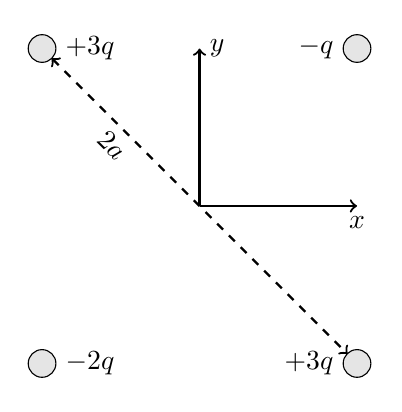
\begin{tikzpicture}
        %% coordinates
        \draw[thick,->] (0,0) -- (2,0) node[anchor=north] {$x$};
        \draw[thick,->] (0,0) -- (0,2) node[anchor=west] {$y$};
        %% Charges
        \draw[fill=white!90!black] (-2,-2) circle (5pt) node [anchor=west,xshift=5pt] {$-2q$};
        \draw[fill=white!90!black] (-2,+2) circle (5pt) node [anchor=west,xshift=5pt] {$+3q$};
        \draw[fill=white!90!black] (+2,+2) circle (5pt) node [anchor=east,xshift=-5pt] {$-q$};
        \draw[fill=white!90!black] (+2,-2) circle (5pt) node [anchor=east,xshift=-5pt] {$+3q$};
        %% 2a
        \draw[thick,dashed,<->] (-1.88,1.88) -- (1.88,-1.88) node[pos=0.25,anchor=north,rotate=-45] {$2a$};
    \end{tikzpicture}
    \end{center}
    What is the total electric field at the center of the square?
    \begin{choices}
        \wrongchoice{$\dfrac{kq}{a^2}$ at an angle \ang{45} above the $+x$ axis.}
      \correctchoice{$\dfrac{kq}{a^2}$ at an angle \ang{45} below the $-x$ axis.}
        \wrongchoice{$\dfrac{3 kq}{a^2}$ at an angle \ang{45} above the $-x$ axis.}
        \wrongchoice{$\dfrac{3 kq}{a^2}$ at an angle \ang{45} below the $+x$ axis.}
        \wrongchoice{$\dfrac{9 kq}{a^2}$ at an angle \ang{45} above the $+x$ axis.}
    \end{choices}
\end{question}
}

\newcommand{\olympiadNinetySevenQTwentyFour}{
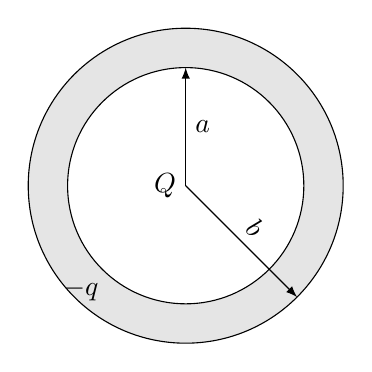
\begin{tikzpicture}
    %% spherical shell
    \draw[fill=white!90!black] (0,0) circle (2cm);
    \draw[fill=white] (0,0) circle (1.5cm);
    %% radius
    \draw[-latex] (0,0) -- (90:1.5) node[pos=0.5,anchor=west] {$a$};
    \draw[-latex] (0,0) -- (315:2.0) node[pos=0.5,anchor=south,rotate=-45] {$b$};
    %% -q and Q
    \node[anchor=east] (0,0) {$Q$};
    \node[anchor=center] at (225:1.88) {$-q$};
\end{tikzpicture}
}

\element{aapt}{ %% Olympiad-D1
\begin{question}{olympiad-1997-q24}
    %Both questions 24 and 25 refer to the system shown in the diagram.
    A spherical shell with an inner surface of radius $a$ and an outer surface of radius $b$ is made of conducting material.
    A point charge $+Q$ is placed at the center of the spherical shell and a total charge $-q$ is placed on the shell.
    \begin{center}
        \olympiadNinetySevenQTwentyFour
    \end{center}
    %% start question
    How is the charge $-q$ distributed after it has reached equilibrium?
    \begin{choices}
        \wrongchoice{Zero charge on the inner surface, $-q$ on the outer surface.}
        \wrongchoice{$-Q$ on the inner surface, $-q$ on the outer surface.}
      \correctchoice{$-Q$ on the inner surface, $-q+Q$ on the outer surface.}
        \wrongchoice{$+Q$ on the inner surface, $-q-Q$ on the outer surface.}
        \wrongchoice{The charge $-q$ is spread uniformly between the inner and outer surface.}
    \end{choices}
\end{question}
}

\element{aapt}{ %% Olympiad-D1
\begin{question}{olympiad-1997-q25}
    %Both questions 24 and 25 refer to the system shown in the diagram.
    A spherical shell with an inner surface of radius $a$ and an outer surface of radius $b$ is made of conducting material.
    A point charge $+Q$ is placed at the center of the spherical shell and a total charge $-q$ is placed on the shell.
    \begin{center}
        \olympiadNinetySevenQTwentyFour
    \end{center}
    %% start question
    Assume that the electrostatic potential is zero at an infinite distance from the spherical shell.
    What is the electrostatic potential at a distance $R$ from the center of the shell,
        where $b^3 R^3 a$?
    \begin{multicols}{3}
    \begin{choices}
        \wrongchoice{zero}
        \wrongchoice{$k\dfrac{Q}{a}$}
        \wrongchoice{$k\dfrac{Q}{R}$}
        \wrongchoice{$k\dfrac{Q-q}{R}$}
      \correctchoice{$k\dfrac{Q-q}{b}$}
    \end{choices}
    \end{multicols}
\end{question}
}


%% PhysicsOlympiad 1996
%%----------------------------------------
\element{aapt}{ %% Olympiad-D1
\begin{question}{olympiad-1996-q23}
    The accompanying figure shows two concentric spherical shells isolated from each other. 
    The smaller shell has radius $b$ and net charge $+Q$.
    The larger shell has radius $2b$ and an equal net charge $+Q$. 
    \begin{center}
    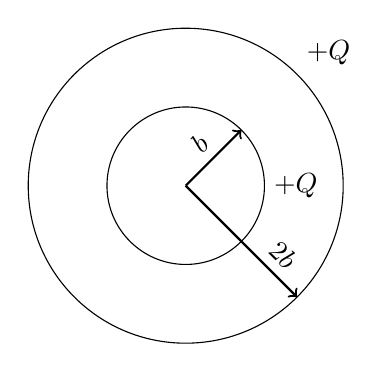
\begin{tikzpicture}
        %% small sphere
        \draw (0,0) circle (1cm);
        \draw[thick,->] (0,0) -- (45:1) node[pos=0.5,anchor=south,rotate=45] {$b$};
        \node[anchor=west] at (0:1) {$+Q$};
        %% large sphere
        \draw (0,0) circle (2cm);
        \draw[thick,->] (0,0) -- (315:2) node[pos=0.75,anchor=south,rotate=-45] {$2b$};
        \node[anchor= south west] at (45:2) {$+Q$};
    \end{tikzpicture}
    \end{center}
    If $R$ is the distance from the common center,
        the highest electric field magnitude $E$ occurs:
    \begin{choices}
        \wrongchoice{only at $R=0$, where $E$ is infinite.}
        \wrongchoice{anywhere $R<b$, where $E$ is constant}
      \correctchoice{immediately outside the smaller ($R=b$) shell.}
        \wrongchoice{immediately outside the larger ($R=2b$) shell.}
        \wrongchoice{far away from the shells; $E$ increases with distance.}
    \end{choices}
\end{question}
}

\element{aapt}{ %% Olympiad-D1
\begin{question}{olympiad-1996-q24}
    An infinite conducting plate of thickness \SI{0.0200}{\meter} is surrounded by a uniform field $E=\SI{400}{\volt\per\meter}$ directed left to right. 
    %See the figure to the right. 
    \begin{center}
    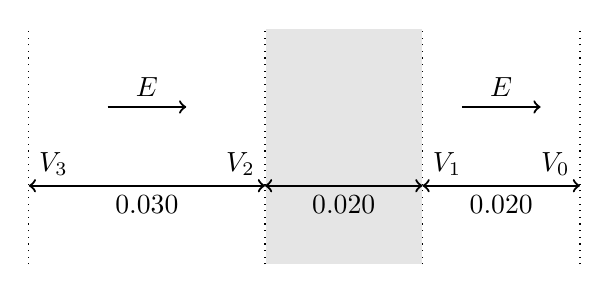
\begin{tikzpicture}
        %% conducting plate
        \draw[white,fill=white!90!black] (-1,0) rectangle (1,3);
        %% boundaries
        \draw[dotted] (-4,0) -- (-4,3);
        \draw[dotted] (-1,0) -- (-1,3);
        \draw[dotted] (+1,0) -- (+1,3);
        \draw[dotted] (+3,0) -- (+3,3);
        % E field
        \draw[thick,->] (-3,2) -- (-2,2) node[pos=0.5,anchor=south] {$E$};
        \draw[thick,->] (+1.5,2) -- (+2.5,2) node[pos=0.5,anchor=south] {$E$};
        % Voltage
        \draw[thick,<->] (-4,1) -- (-1,1)   
            node[pos=0.0,anchor=south west] {$V_3$}
            node[pos=0.5,anchor=north] {\SI{0.030}{\meter}}
            node[pos=1.0,anchor=south east] {$V_2$};
        \draw[thick,<->] (+1,1) -- (+3,1)   
            node[pos=0.0,anchor=south west] {$V_1$}
            node[pos=0.5,anchor=north] {\SI{0.020}{\meter}}
            node[pos=1.0,anchor=south east] {$V_0$};
        \draw[thick,<->] (-1,1) -- (+1,1)   
            node[pos=0.5,anchor=north] {\SI{0.020}{\meter}};
    \end{tikzpicture}
    \end{center}
    Let the potential $V_0=0$ a distance \SI{0.0200}{\meter} to the right of the plate. 
    What is $V_3$, the potential \SI{0.0300}{\meter} to the left of the plate?
    \begin{multicols}{3}
    \begin{choices}
        \wrongchoice{\SI{-28}{\volt}}
        \wrongchoice{\SI{-20}{\volt}}
        \wrongchoice{\SI{+12}{\volt}}
      \correctchoice{\SI{+20}{\volt}}
        \wrongchoice{\SI{+28}{\volt}}
    \end{choices}
    \end{multicols}
\end{question}
}

\element{aapt}{ %% Olympiad-D1
\begin{question}{olympiad-1996-q25}
    A sphere of radius $a$ has uniform charge density $\rho$.
    A spherical cavity of radius $c$ is formed in the sphere. 
    The cavity is centered a distance $b$ ($b>c$) from the center of the sphere. 
    \begin{center}
    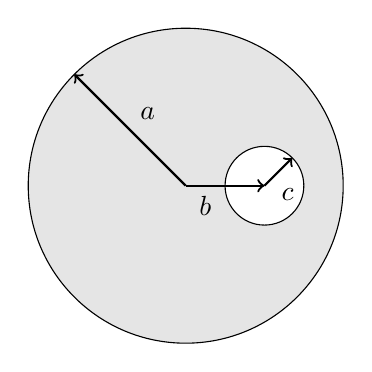
\begin{tikzpicture}
        %% spherical cavity
        \draw[fill=white!90!black] (0,0) circle (2cm);
        \draw[fill=white] (1,0) circle (0.5cm);
        %% radius
        \draw[thick,->] (0,0) -- (135:2) node[pos=0.5,anchor=south west] {$a$};
        \draw[thick,->] (0,0) -- (1,0) node[pos=0.25,anchor=north] {$b$};
        \draw[thick,->] (1,0) -- ++(45:0.5) node[pos=0.25,anchor=north west] {$c$};
    \end{tikzpicture}
    \end{center}
    What is the magnitude of the electric field at the center of the cavity?
    \begin{multicols}{2}
    \begin{choices}
      \correctchoice{$\dfrac{\rho b}{3\varepsilon_0}$}
        \wrongchoice{$\dfrac{\rho a^3}{3\varepsilon_0 b^2}$}
        \wrongchoice{$\dfrac{\rho \left(a^3-c^3\right)}{3\varepsilon_0 b^2}$}
        \wrongchoice{$\dfrac{\rho}{3\varepsilon_0} \left(b-\dfrac{c^3}{2b^2}\right)$}
        \wrongchoice{$\dfrac{\rho}{3\varepsilon_0} \left(b-\dfrac{c^3}{b^2}\right)$}
        %\wrongchoice{$\dfrac{\rho \left(b-\dfrac{c^3}{2b^2}\right)}{3\varepsilon_0}$}
        %\wrongchoice{$\dfrac{\rho \left(b-\dfrac{c^3}{b^2}\right)}{3\varepsilon_0}$}
    \end{choices}
    \end{multicols}
\end{question}
}

\element{aapt}{ %% Olympiad-D1
\begin{question}{olympiad-1996-q26}
    As shown in the diagram below, two fixed charges,
    \begin{center}
    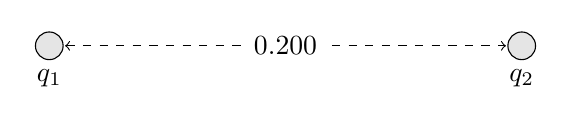
\begin{tikzpicture}
        %% charges
        \draw[fill=white!90!black] (-3,0) circle (5pt) node[anchor=north,yshift=-5pt] {$q_1$};
        \draw[fill=white!90!black] (+3,0) circle (5pt) node[anchor=north,yshift=-5pt] {$q_2$};
        %% distance
        \draw[dashed,<->] (-2.8cm,0) -- (+2.8cm,0) node[pos=0.5,anchor=center,fill=white] {\SI{0.200}{\meter}};
    \end{tikzpicture}
    \end{center}
    $q_1 = \SI{+1.00}{\micro\coulomb}$ and $q_2=\SI{-4.00}{\micro\coulomb}$, are \SI{0.200}{\meter} apart. 
    Where is the total field zero?
    \begin{choices}
        \wrongchoice{\SI{0.40}{\meter} to the right of $q_1$}
        \wrongchoice{\SI{0.13}{\meter} to the right of $q_1$}
        \wrongchoice{\SI{0.1}{\meter} to the right of $q_1$}
        \wrongchoice{\SI{0.067}{\meter} to the left of $q_1$}
      \correctchoice{\SI{0.20}{\meter} to the left of $q_1$}
    \end{choices}
\end{question}
}


%% PhysicsOlympiad 1995
%%----------------------------------------
\element{aapt}{ %% Olympiad-D1
\begin{question}{olympiad-1995-q26}
    The accompanying figure shows two concentric spherical shells isolated from each other.
    \begin{center}
    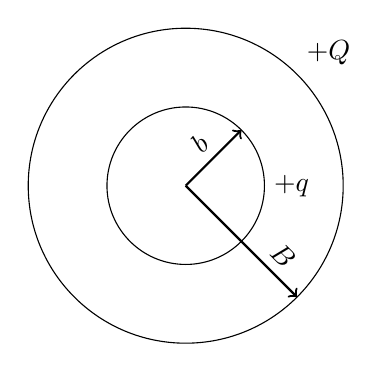
\begin{tikzpicture}
        %% small sphere
        \draw (0,0) circle (1cm);
        \draw[thick,->] (0,0) -- (45:1) node[pos=0.5,anchor=south,rotate=45] {$b$};
        \node[anchor=west] at (0:1) {$+q$};
        %% large sphere
        \draw (0,0) circle (2cm);
        \draw[thick,->] (0,0) -- (315:2) node[pos=0.75,anchor=south,rotate=-45] {$B$};
        \node[anchor= south west] at (45:2) {$+Q$};
    \end{tikzpicture}
    \end{center}
    The smaller shell has radius $b$ and net charge $+q$.
    The larger shell has radius $B$ and net charge $+Q$.
    Assume that the potential is zero at an infinite distance from the shells.
    If $R$ is the distance from the common center,
        the highest electric potential $V$ occurs:
    \begin{choices}
        \wrongchoice{only at $R=0$, where $V$ is infinite}
      \correctchoice{anywhere $R\geq b$, where $V$ is constant}
        \wrongchoice{in the region $b < R < B$.}
        \wrongchoice{immediately outside the larger shell; $V$ is zero everywhere within it.}
        \wrongchoice{far away from the shells; $V$ increases with distance.}
    \end{choices}
\end{question}
}


%% PhysicsOlympiad 1994
%%----------------------------------------
\newcommand{\aaptOlympiadNinetyFourQTwentyFour}{
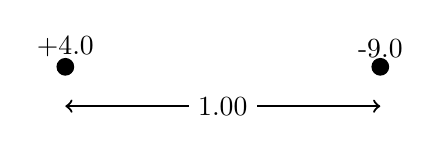
\begin{tikzpicture}
    %% charges
    \draw[fill] (-2,0) circle (3pt) node[anchor=south] {\SI{+4.0}{\micro\coulomb}};
    \draw[fill] (+2,0) circle (3pt) node[anchor=south] {\SI{-9.0}{\micro\coulomb}};
    %% length
    \draw[thick,<->] (-2,-0.5) -- (2,-0.5) node[pos=0.5,anchor=center,fill=white] {\SI{1.00}{\meter}};
\end{tikzpicture}
}

\element{aapt}{ %% Olympiad-D1
\begin{question}{olympiad-1994-q24}
    %Refer to the following information for the next two questions.
    Two point charges of \SI{+4.00}{\micro\coulomb} and \SI{-9.00}{\micro\coulomb} are placed \SI{1.00}{\meter} apart,
        as shown in the accompanying figure.
    \begin{center}
        \aaptOlympiadNinetyFourQTwentyFour
    \end{center}
    Assume the potential goes to zero as $R$ goes to infinity.
    %% start question
    The total electric field due to the two charges is zero at a point:
    \begin{choices}
        \wrongchoice{\SI{3.00}{\meter} to the right of the \SI{-9.00}{\micro\coulomb} charge.}
        \wrongchoice{\SI{0.40}{\meter} to the right of the \SI{+4.00}{\micro\coulomb} charge.}
        \wrongchoice{\SI{0.31}{\meter} to the right of the \SI{+4.00}{\micro\coulomb} charge.}
        \wrongchoice{\SI{0.80}{\meter} to the left of the \SI{+4.00}{\micro\coulomb} charge.}
      \correctchoice{\SI{2.00}{\meter} to the left of the \SI{+4.00}{\micro\coulomb} charge.}
    \end{choices}
\end{question}
}

\element{aapt}{ %% Olympiad-D1
\begin{question}{olympiad-1994-q25}
    %Refer to the following information for the next two questions.
    Two point charges of \SI{+4.00}{\micro\coulomb} and \SI{-9.00}{\micro\coulomb} are placed \SI{1.00}{\meter} apart,
        as shown in the accompanying figure.
    \begin{center}
        \aaptOlympiadNinetyFourQTwentyFour
    \end{center}
    Assume the potential goes to zero as $R$ goes to infinity.
    %% start question
    How much work is done moving the \SI{-9.00}{\micro\coulomb} charge from its original position to a new position \SI{2.00}{\meter} from the \SI{+4.00}{\micro\coulomb} charge?
    \begin{multicols}{3}
    \begin{choices}
        \wrongchoice{\SI{-0.324}{\joule}}
        \wrongchoice{\SI{-0.081}{\joule}}
      \correctchoice{\SI{+0.162}{\joule}}
        \wrongchoice{\SI{+0.243}{\joule}}
        \wrongchoice{\SI{+0.486}{\joule}}
    \end{choices}
    \end{multicols}
\end{question}
}

\element{aapt}{ %% Olympiad-D1
\begin{question}{olympiad-1994-q26}
    A point charge $Q$ is placed at the center of a spherical conducting shell,
        the shaded part of the accompanying figure.
    A total charge of $-q$ is placed on the shell.
    \begin{center}
    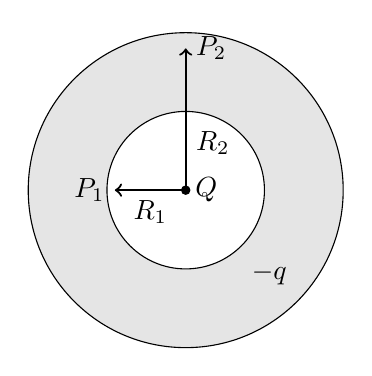
\begin{tikzpicture}
        %% Inner and outer
        \draw[fill=white!90!black] (0,0) circle (2cm);
        \draw[fill=white] (0,0) circle (1cm);
        %% charge
        \draw[fill] (0,0) circle (1.5pt) node[anchor=west] {$Q$};
        \node[anchor=center] at (315:1.5) {$-q$};
        %% Radius
        \draw[thick,->] (0,0) -- (90:1.8cm)
            node[pos=0.33,anchor=west] {$R_2$}
            node[pos=1.00,anchor=west] {$P_2$};
        \draw[thick,->] (0,0) -- (180:0.9cm)
            node[pos=0.50,anchor=north] {$R_1$}
            node[pos=1.00,anchor=east] {$P_1$};
    \end{tikzpicture}
    \end{center}
    The magnitude of the electric field at point $P_1$ a distance $R_1$ from the center is \rule[-0.1pt]{4em}{0.1pt}.
    The magnitude of the electric field at point $P_2$ a distance $R_2$ from the center is \rule[-0.1pt]{4em}{0.1pt}.
    \begin{multicols}{2}
    \begin{choices}
      \correctchoice{zero; zero}
        \wrongchoice{$k\dfrac{Q}{R_1^2}$; zero}
        \wrongchoice{$k\dfrac{Q-q}{R_1^2}$; zero}
        \wrongchoice{zero; $k\dfrac{Q-q}{R_2^2}$}
        \wrongchoice{$k\dfrac{Q-q}{R_1^2}$; $k\dfrac{Q-q}{R_2^2}$}
    \end{choices}
    \end{multicols}
\end{question}
}



\endinput


